\chapter{Architettura del progetto}

\section{Overview}
Come input alla realizzazione della nostra applicazione, siamo partiti da una demo offerta direttamente da MediaPipe. In questa applicazione viene data la possibilità all'utente di visualizzare la mappatura delle proprie mani scegliendo diverse modalità di acquisizione dell'immagine.
Oltre a file ausiliari come il \textit{manifest} o gli \textit{xml} di configurazione, il cuore del progetto è rappresentato da 3 file nel package \texttt{hands/ja-} \texttt{va/com/google/mediapipe/examples/hands}.
\begin{figure}[H]
    \centering
    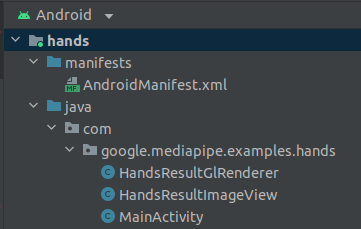
\includegraphics[width=0.5\textwidth]{images/struct_demo.png}
\end{figure}
\noindent Ovviamente, \texttt{MainActivity} corrisponde all'entry point dell'applicazione ed eredita infatti da \texttt{AppCompatActivity}.\\
\\
\noindent Nonostante noi ci siamo concentrati solo sull'input da streaming video, l'applicazione mette a disposizione 3 diverse modalità di acquisizione dell'input, rappresentate dall'enumerativo \texttt{InputSource} all'interno del quale troviamo \texttt{CAMERA}, \texttt{VIDEO} e \texttt{IMAGE}.\\


\section{Struttura del progetto}
\begin{figure}[H]
    \centering
    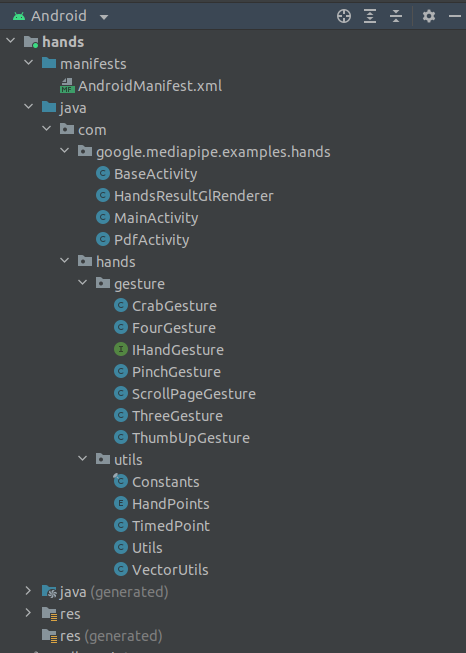
\includegraphics[width=0.8\textwidth]{images/struct_progetto.png}
\end{figure}
All'interno del package \texttt{hands/java/com/google/mediapipe/examples/hands} abbiamo potuto eliminare la classe \texttt{HandsResultImageView}, utile solo con acquisizione dell'input tramite immagine statica; mentre la classe \texttt{HandsResultGlRenderer}, per il rendering su schermo, è stata lasciata sostanzialmente inalterata.\\
Sono state invece applicate delle modifiche consistenti alla classe \texttt{MainActivity} (aggiungendo anche altre due classi \textit{Activity}) per implementare la logica applicativa.\\


\subsection{BaseActivity, MainActivity e PdfActivity}
Mentre prima era \texttt{MainActivity} ad ereditare da \texttt{AppCompatActivity}, ora questo avviene per \texttt{BaseActivity}, da cui erediteranno poi la classe \texttt{PdfActivity} e la nuova \texttt{MainActivity}.\\
Abbiamo scelto di adottare questa strategia implementativa per suddividere in modo chiaro e pulito le funzionalità esposte dalle due classi:
\begin{itemize}
    \item \texttt{MainActivity}: si occupa di definire il layout dell'applicazione nel caso in cui si voglia visualizzare su tutto lo schermo la propria mano, con alcune \texttt{TextView} per mostrare il riconoscimento di determinate \textbf{gesture}.
    \item \texttt{PdfActivity}: corrisponde al cuore dell'applicazione, definendo un layout nel quale è presente un file \texttt{pdf} da leggere ed una piccola vista della fotocamera interna dello smartphone. Quest'ultima ha lo scopo di mostrare all'utente il movimento della propria mano, tramite la quale avrà la possibilità di interagire con il file.
\end{itemize}
\noindent Entrambe le \textit{activities} hanno quindi lo scopo di mostrare la mano ed il riconoscimento di gesture, la prima \textit{"loggando"} l'eventuale riconoscimento, la seconda interagendo con il pdf.\\
Per fare questo, all'interno di ognuna, viene definito un \textbf{listener} che controlla continuamente l'eventuale associazione di un movimento della mano ad una gesture. Sono state infatti create 6 classi, una per gesture, che si occupano di effettuare il controllo sulla base dei \textbf{landmarks} passati in input dalle \textit{activities}.\\
\\
Prima di concentrarci su questE classi, di seguito vengono esposte caratteristiche più dettagliate di ognuna delle \textit{activitites} presentate sopra.

\subsubsection{BaseActivity}
Questa classe funge da contenitore per tutte quelle variabili e funzioni comuni sia a \texttt{MainActivity} sia a \texttt{PdfActivity} (perciò dichiarate con la clausola \texttt{protected}). Questa permette di evitare la ridondanza di codice.\\

\paragraph{Variabili} Alcune delle variabili comuni definite sono:
\begin{itemize}
    \item \texttt{Hands}, tramite la quale viene recuperato il \textbf{listener} nominato sopra, da cui poi otteniamo i risultati del mapping effettuato dalla pipeline di riconoscimento di MediaPipe.
    \item \texttt{InputSource}, che rappresenta la modalità di acquisizione dell'immagine (da noi sarà sempre \texttt{CAMERA}).
    \item \texttt{CameraInput}, che rappresenta la ricezione dell'input dalla fotocamera.
\end{itemize}
\noindent Abbiamo poi \texttt{SolutionGlSurfaceView$<$HandsResult$>$} e \texttt{HandsResultGlRenderer} per la definizione del layout e per il rendering.\\ 
Infine, sono presenti le istanze di tutte quelle classi che effettuano il rilevamento delle gesture, che, come detto in precedenza, sono necessarie ad entrambe le \texttt{activities}, anche se con scopi diversi.

\paragraph{Metodi} Essendo che questa classe eredita da \texttt{AppCompatActivity}, è necessario effettuare l'\texttt{override} dei seguenti metodi:
\begin{itemize}
    \item \texttt{onCreate}, accetta un \texttt{Bundle} in input, utilizzato per chiamare la \texttt{onCreate} della classe estesa. In Android Studio i \textit{Bundle} si utilizzano solitamente per il passaggio di dati da un attività all'altra: in questo caso abbiamo un istanza di uno stato salvato precedentemente (e.g. l'applicazione era stata messa in background). All'interno di questa funzione è solito definire il layout della pagina, ma abbiamo scelto di farlo solo nelle \textit{activities specializzate} che erediteranno da \texttt{BaseActivity}.
    \item \texttt{onPause}, nella quale viene chiamata la \texttt{onPause} della classe estesa per poi nascondere la visibilità del layout (\texttt{glSurfaceView}) e fermare infine il flusso video in input dalla fotocamera.
    \item \texttt{onResume}, dove dopo essere stata chiamata la \texttt{onResume} della classe estesa, si istanzia un nuovo \texttt{CameraInput} (passandogli l'\textit{activity} corrente) per poi settare un nuovo \textit{FrameListener}. Successivamente viene utilizzata l'istanza di \texttt{SolutionGlSurfaceView<HandsResult>} per chiamare il metodo interno \texttt{post}, passandogli la funzione interna \texttt{startCamera()} (il cui scopo è quello di inizializzare lo streaming video). In questo modo, tramite la \texttt{post} ereditata dalla classe \texttt{View}, viene eseguita la funzione passata ed esposto l'output nell'interfaccia utente.
\end{itemize}
\noindent Sono presenti poi ulteriori funzioni che vengono utilizzate da \texttt{MainActivity} e \texttt{PdfActivity} per inizializzare la pipeline di acquisizione dell'input e per terminarla. Verranno analizzate in seguito.



\subsubsection{MainActivity}
Abbiamo detto che lo scopo di questa \textit{activity} è quello di mostrare su schermo l'eventuale riconoscimento di determinate gesture. Perciò, oltre alle variabili definite nella classe estesa, le uniche variabili globali presenti sono una serie \texttt{TextView}, una per ogni gesture.\\
Viene effettuato l'\texttt{override} delle funzioni ereditate da \texttt{AppCompatActivity} e, mentre \texttt{onPause} e \texttt{onResume} chiamano solamente le relative funzioni della classe \texttt{BaseActivity}, la \texttt{onCreate} si occupa inoltre di \underline{inizializzare lo streaming video} e di definire il layout della pagina, istanziando anche un nuovo bottone per accedere alla funzionalità di interazione coi file \texttt{pdf}.\\
\\
Per quanto riguarda l'inizializzazione dello streaming video, vengono utilizzate due funzioni:
\begin{itemize}
    \item \texttt{setupLiveDemoUiComponents}, all'interno della quale viene definito un bottone per attivare lo streaming che, una volta cliccato, causerà la chiamata alla stessa funzione della classe estesa (il cui scopo è quello di fermare la pipeline di acquisizione attuale (nel caso in cui la modalità di acquisizione sia diversa da \texttt{CAMERA})). Successivamente, viene chiamata la funzione che implementa effettivamente la pipeline, mostrata qui sotto.
    \item \texttt{setupStreamingModePipeline}, questa funzione è divisa sostanzialmente in 3 parti, oltre ad una preliminare nella quale vengono inizializzate le \texttt{TextView}. \begin{enumerate}
        \item chiamata alla funzione \texttt{firstSetupStreamingModePipeline} di \texttt{BaseActivity} che crea delle nuove istanze di \texttt{HandsResultGlRenderer}, \texttt{Hands} e \texttt{glSurfaceView}. Tramite essa inizia lo streaming dalla fotocamera e, concorrentemente, la pipeline per il mapping dei \textbf{landamrks} della mano.
        \item settato il \textbf{listener} per il riconoscimento delle gesture, all'interno del quale vengono effettuate delle chiamate alle classi per il controllo e mostrato l'eventuale riconoscimento colorando le \texttt{Textview} definite prima.
        \item chiamata alla funzione \texttt{lastSetupStreamingModePipeline} di \texttt{BaseActivity} che chiama il metodo \texttt{post} di \texttt{glSurfaceView} visto in precedenza e definisce il nuovo \texttt{FrameLayout} con i dati trovati nella fase precedente.
    \end{enumerate}
\end{itemize}


\subsubsection{PdfActivity}
Il funzionamento di questa classe è analogo a quella mostrata in precedenza. Viene ovviamente differenziato il layout della pagina e, all'interno del \textit{listener} della funzione \texttt{setupStreamingModePipeline}, vengono associate le varie gesture riconosciute ad azioni che permettono di interagire con il file \texttt{pdf} che si sta visualizzando.